\documentclass[../main.tex]{subfiles}
\graphicspath{{\subfix{../img/}}}

\begin{document}

\section{Gating Functions and Parameters for Implemented Models} \label{appendix:functions_and_parameters}

\subsection{Wang 1994}

The model and corresponding parameters were obtained from \cite{wangMultipleDynamicalModes1994}.
The model contains six types of currents (i.e. currents passing through particular ion channel):
\begin{itemize}
    \item T-type calcium current: $I_{T}(V)=g_T \cdot s_\infty^3(V) \cdot h \cdot (V - V_{Ca})$
    \begin{itemize}[label=\textopenbullet]
        \item $s_\infty(V)=1/(1+\exp(-(V+65)/7.8))$
        \item $\frac{dh}{dt}(V)=2\cdot(h_\infty - h)/\tau_h$
        \item $h_\infty(V)=\frac{1}{1 + \exp((V + 79)/5)}$
        \item $\tau_h(V)=h_\infty \cdot \exp((V + 162.3)/17.8) + 20$
    \end{itemize}
    \item Sag (or, h-) current: $I_{H}=g_{\text{H}} \cdot H^2 \cdot (V - V_{\text{H}})$
    \begin{itemize}[label=\textopenbullet]
        \item $\frac{dH}{dt}(V)=(H_\infty(V) - H)/\tau_{H}(V)$
        \item $H_\infty(V)=\dfrac{1}{1 + \exp((V + 69)/7.1)}$
        \item $\tau_{\text{H}}(V)=\frac{1000}{\exp((V + 66.4)/9.3) + \exp(-(V + 81.6)/13)}$
    \end{itemize}
    \item Hodgkin and Huxley potassium current: $I_{HH,K}=g_{\text{hhK}} \cdot n^4 \cdot (V - V_K)$
    \begin{itemize}[label=\textopenbullet]
        \item $\frac{dn}{dt}(V)=\frac{200}{7} \cdot (n_\infty(V) - n)/\tau_n(V)$
        \item $\alpha_n(V)=-0.01 \cdot (V + 35.7)/[\exp(-0.1 \cdot (V + 35.7)) - 1]$
        \item $\beta_n(V)=0.125 \cdot \exp(-(V + 45.7)/80)$
        \item $n_\infty(V)=\frac{\alpha_n(V)}{\alpha_n(V) + \beta_n(V)}$
        \item $\tau_n(V)=\dfrac{1}{\alpha_n(V) + \beta_n(V)}$
    \end{itemize}
    \item Hodgkin and Huxley sodium current: $I_{HH,Na}(V)=g_{\text{Na}} \cdot m_\infty^3 \cdot (0.85 - n) \cdot (V - V_{\text{Na}})$
    \item Persistent sodium current: $I_{NaP}(V)=g_{NaP} \cdot m_{\infty,Nap}^3 \cdot (V - V_{\text{Na}})$
    \item Leak Current: $I_L(V)=g_{\text{Leak}} \cdot (V - V_{\text{Leak}})$
\end{itemize}

Dafault parameters:
$c_{\text{Membr}}=1$ $\mu F/cm^2$,
$g_T=1$ $mS/cm^2$,
$v_{Ca}=120$ $mV$,
$g_{\text{G}}=0.04$ $mS/cm^2$,
$v_{\text{G}}=-40$ $mV$,
$g_{\text{HHK}}=30$ $mS/cm^2$,
$v_K=-80$ $mV$,
$g_{\text{Na}}=42$ $mS/cm^2$,
$v_{\text{Na}}=55$ $mV$,
$g_{\text{NaP}}=9$ $mS/cm^2$,
$g_{\text{Leak}}=0.12$ $mS/cm^2$,
$v_{\text{Leak}}=-70$ $mV$,
$I_{\text{ext}}=-1.6$ $\mu A / cm1 2$,

\begin{figure}[!t]
    \centering
    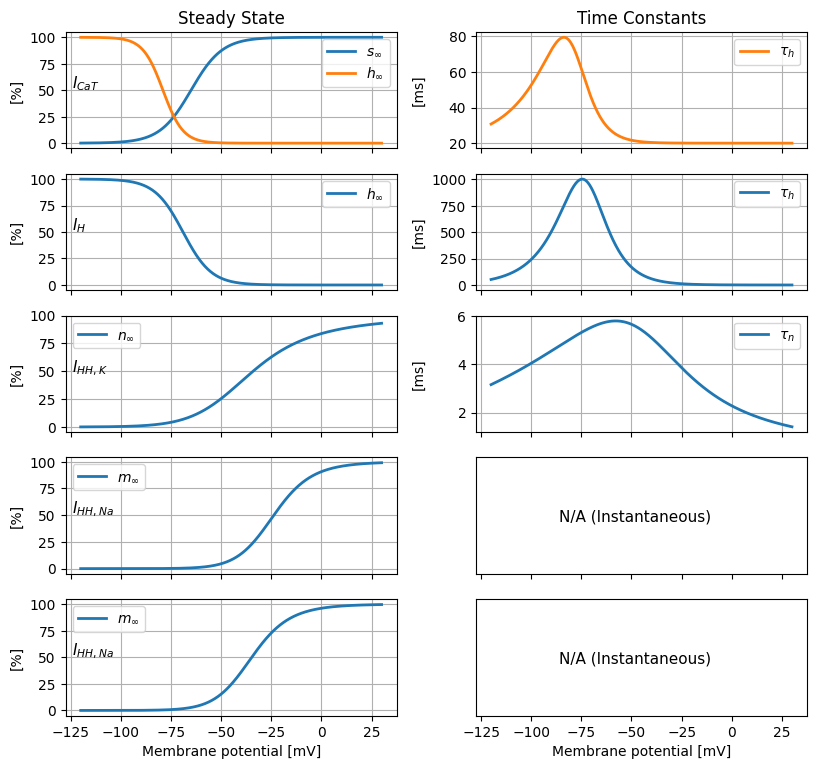
\includegraphics[width=\linewidth]{../img/model_kinetics/kinetics_wang.png}
    \caption[Wang: Steady state activation and inactivation functions, and corresponding time constants]{
        \textbf{Wang: Steady state activation and inactivation functions, and corresponding time constants}. Note, that the negative values of the $I_{HH,Na}$ inactivation gate results from the simplification of the dynamics by assuming litear relationship between the inactivation gate of the HH sodium and activation gate of HH potassium channels \parencite{wangMultipleDynamicalModes1994}.
    }
    \label{fig:kinetic_plots_wang1994}
\end{figure}
\clearpage

\FloatBarrier

\newpage
\subsection{Goldman et. al. 2001}

The model and parameters adapted from \parencite{franciRobustTunableBursting2018}.
The model contains six types of currents (i.e. currents passing through particular ion channel):
\begin{itemize}

    \item Fast sodium current (INa\textsubscript{T}): 
    $I_{\text{NaT}} = g_{\text{nat}} \cdot m^3 \cdot h \cdot (V - V_{\text{Na}})$
    \begin{itemize}[label=\textopenbullet]
        \item $\frac{dm}{dt} = \frac{m_\infty(V) - m}{\tau_m(V)}$
        \item $m_\infty(V) = \dfrac{1}{1 + \exp\left(\frac{V + 25.5}{-5.29}\right)}$
        \item $\tau_m(V) = 1.32 - \dfrac{1.26}{1 + \exp\left(\frac{V + 120}{-25}\right)}$
        \item $\frac{dh}{dt} = \frac{h_\infty(V) - h}{\tau_h(V)}$
        \item $h_\infty(V) = \dfrac{1}{1 + \exp\left(\frac{V + 48.9}{5.18}\right)}$
        \item $\tau_h(V) = \dfrac{0.67}{1 + \exp\left(\frac{V + 62.9}{-10}\right)} \cdot \left(1.5 + \dfrac{1}{1 + \exp\left(\frac{V + 34.9}{3.6}\right)}\right)$
    \end{itemize}

    \item T-type calcium current:
    $I_{\text{CaT}}(V) = g_{\text{cat}} \cdot m^3 \cdot h \cdot (V - V_{\text{Ca}})$
    \begin{itemize}[label=\textopenbullet]
        \item $\frac{dm}{dt} = \frac{m_\infty(V) - m}{\tau_m}$,\quad $m_\infty(V) = \dfrac{1}{1 + \exp\left(\frac{V + 27.1}{-7.2}\right)}$
        \item $\tau_m(V) = 21.7 - \dfrac{21.3}{1 + \exp\left(\frac{V + 68.1}{-20.5}\right)}$
        \item $\frac{dh}{dt}(V) = \frac{h_\infty - h}{\tau_h}$,\quad $h_\infty = \dfrac{1}{1 + \exp\left(\frac{V + 32.1}{5.5}\right)}$
        \item $\tau_h(V) = 105 - \dfrac{9.8}{1 + \exp\left(\frac{V + 55}{-16.9}\right)}$
    \end{itemize}

    \item Slow calcium current:
    $I_{\text{CaS}}(V) = g_{\text{cas}} \cdot m^3 \cdot h \cdot (V - V_{\text{Ca}})$
    \begin{itemize}[label=\textopenbullet]
        \item $\frac{dm}{dt} = \frac{m_\infty - m}{\tau_m}$,\quad $m_\infty(V) = \dfrac{1}{1 + \exp\left(\frac{V + 33}{-8.1}\right)}$
        \item $\tau_m(V) = 1.4 + \dfrac{7}{\exp\left(\frac{V + 27}{10}\right) + \exp\left(\frac{V + 70}{-13}\right)}$
        \item $\frac{dh}{dt}(V) = \frac{h_\infty(V) - h}{\tau_h(V)}$,\quad $h_\infty(V) = \dfrac{1}{1 + \exp\left(\frac{V + 60}{6.2}\right)}$
        \item $\tau_h(V) = 60 + \dfrac{150}{\exp\left(\frac{V + 55}{9}\right) + \exp\left(\frac{V + 65}{-16}\right)}$
    \end{itemize}

    \item A-type potassium current:
    $I_{A}(V) = g_{a} \cdot m^3 \cdot h \cdot (V - V_{K})$
    \begin{itemize}[label=\textopenbullet]
        \item $\frac{dm}{dt} = \frac{m_\infty(V) - m}{\tau_m(V)}$,\quad $m_\infty(V) = \dfrac{1}{1 + \exp\left(\frac{V + 27.2}{-8.7}\right)}$
        \item $\tau_m(V) = 11.6 - \dfrac{10.4}{1 + \exp\left(\frac{V + 32.9}{-15.2}\right)}$
        \item $\frac{dh}{dt} = \frac{h_\infty(V) - h}{\tau_h(V)}$,\quad $h_\infty(V) = \dfrac{1}{1 + \exp\left(\frac{V + 56.9}{4.9}\right)}$
        \item $\tau_h(V) = 38.6 - \dfrac{29.2}{1 + \exp\left(\frac{V + 38.9}{-26.5}\right)}$
    \end{itemize}

    \item Calcium-dependent potassium current:
    $I_{KCa}(V) = g_{\text{kca}} \cdot m^4 \cdot (V - V_K)$
    \begin{itemize}[label=\textopenbullet]
        \item $\frac{dm}{dt} = \frac{m_\infty(V) - m}{\tau_m(V)}$
        \item $m_\infty = \left(\frac{[Ca]}{[Ca] + 3}\right) \cdot \frac{1}{1 + \exp\left(\frac{V + 28.3}{-12.6}\right)}$
        \item $\tau_m = 90.3 - \dfrac{75.1}{1 + \exp\left(\frac{V + 46}{-22.7}\right)}$
    \end{itemize}

    \item Delayed rectifier potassium current:
    $I_{KDR}(V) = g_{\text{kd}} \cdot m^4 \cdot (V - V_K)$
    \begin{itemize}[label=\textopenbullet]
        \item $\frac{dm}{dt} = \frac{m_\infty(V) - m}{\tau_m(V)}$
        \item $m_\infty(V) = \dfrac{1}{1 + \exp\left(\frac{V + 12.3}{-11.8}\right)}$
        \item $\tau_m(V)= 7.2 - \dfrac{6.4}{1 + \exp\left(\frac{V + 28.3}{-19.2}\right)}$
    \end{itemize}

    \item Leak current:
    $I_{\text{leak}}(V) = g_{\text{leak}} \cdot (V - V_{\text{leak}})$

    \item Calcium dynamics:
    \[
    \frac{d[Ca]}{dt} = \frac{-9.4 \cdot (I_{\text{CaT}} + I_{\text{CaS}}) - [Ca] + 0.05}{200}
    \]
\end{itemize}

\vspace{0.5em}
\textbf{Parameters Goldman 1:}
$g_{\text{nat}} = 700$ $mS/cm^2$, $V_{\text{Na}} = 50$ mV, $g_{\text{cat}} = 7$ $mS/cm^2$, $g_{\text{cas}} = 10.5$ $mS/cm^2$,
$V_{\text{Ca}} = 80$ mV, $g_a = 225$ $mS/cm^2$, $g_{\text{kca}} = 25$ $mS/cm^2$, $g_{\text{kd}} = 80$, $V_K = -80$ $mS/cm^2$,
$g_{\text{leak}} = 0.1$ $mS/cm^2$, $V_{\text{leak}} = -50$ mV, $I_{\text{app}} = 2$ $\mu A/cm^2$, $c_m = 1$ $\mu F / cm^2$

\textbf{Parameters Goldman 2:}
$g_{\text{nat}} = 1200$ $mS/cm^2$, $V_{\text{Na}} = 50$ mV, $g_{\text{cat}} = 10$ $mS/cm^2$, $g_{\text{cas}} = 8$ $mS/cm^2$,
$V_{\text{Ca}} = 80$ mV, $g_a = 10$ $mS/cm^2$, $g_{\text{kca}} = 40$, $g_{\text{kd}} = 100$, $V_K = -80$ mV,
$g_{\text{leak}} = 0.1$, $V_{\text{leak}} = -50$ mV, $I_{\text{app}} = 2$ $\mu A/cm^2$, $c = 1$ $\mu F / cm^2$

\begin{figure}[!t]
    \centering
    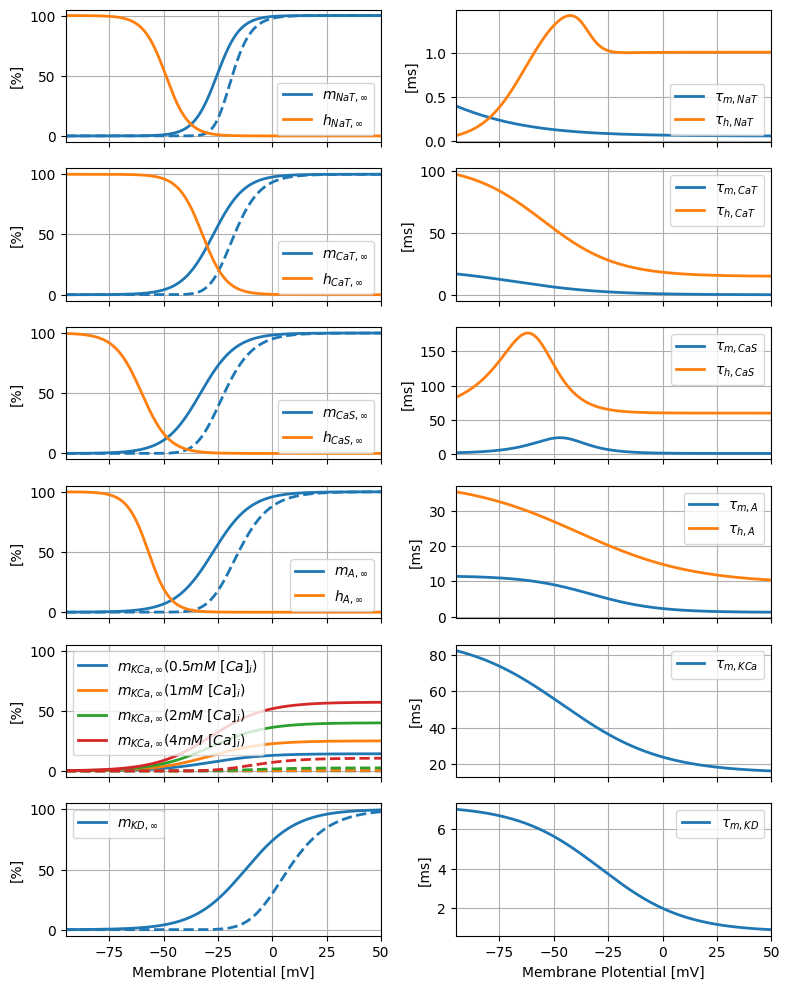
\includegraphics[width=0.9\linewidth]{../img/model_kinetics/goldman.png}
    \caption[Godlman: Steady state activation and inactivation functions, and corresponding time constants]{
        \textbf{Godlman: Steady state activation and inactivation functions, and corresponding time constants} Parameters adapted from \parencite{franciRobustTunableBursting2018}.
    }
    \label{fig:kinetic_plots_goldman}
\end{figure}

\clearpage

\newpage
\subsection{Park et. al. 2021}

The model and parameters adapted from \parencite{parkMathematicalModelSubthalamic2021}.
The model incorporates following currents:
\begin{itemize}
    \item Leak current: $I_L = g_L (V - V_L)$
    \item Spike-generating potassium current: $I_K = g_K n^4 (V - V_K)$
    \item Spike-generating sodium current: $I_{\text{Na}} = g_{\text{Na}} \, m^3 h (V - V_{\text{Na}})$
    \item Persistent sodium current: $I_{\text{NaP}} = g_{\text{NaP}} (V - V_{\text{Na}})$
    \item Calcium-dependent potassium current: $I_{\text{AHP}} = g_{\text{AHP}} \, r^2 (V - V_K)$
    \item \gls{hcn} current: $I_{\text{HCN}} = g_{\text{HCN}} f(V - V_{\text{HCN}})$
    \item A-type potassium current: $I_A = g_A a^2 b (V - V_K)$
    \item T-type low-threshold calcium current: $I_{\text{CaT}} = g_{\text{CaT}} \, p^2 q (V - V_{\text{Ca}})$
    \item n L-type high-threshold calcium current: $I_{\text{CaL}} = g_{\text{CaL}} \, c^2 d_1 d_2 (V - V_{\text{Ca}})$
\end{itemize}

where
\begin{align}
    \frac{dx}{dt} &= \frac{x_\infty(V) - x}{\tau_x(V)}, \quad x \in \{m, h, n, f, a, b, p, q, c, d_1\}, \tag{2} \\
    \frac{dx}{dt} &= \frac{x_\infty([\text{Ca}]) - x}{\tau_x(V)}, \quad x \in \{r, d_2\}, \tag{3} \\
    \frac{d[\text{Ca}]}{dt} &= \frac{\epsilon}{2F} (-I_T - I_{\text{CaL}}) - K_{\text{Ca}}[\text{Ca}], \tag{4}
\end{align}

\begin{align*}
    x_\infty(V) &= \left[ 1 + \exp\left(\frac{V - \theta_{\infty,x}}{\sigma_{\infty,x}}\right) \right]^{-1}, \quad x \in \{m, h, n, f, a, b, p, q, c, d_1\}, \\
    x_\infty([\mathrm{Ca}]) &= \left[ 1 + \exp\left( \frac{[\mathrm{Ca}] - \theta_{\infty,x}}{\sigma_{\infty,x}} \right) \right]^{-1}, \quad x \in \{r, d_2\}, \\
    \tau_x(V) &= \tau_{0,x} + \tau_{1,x} \left[ 1 + \exp\left( -\frac{V - \theta_{1,x}}{\sigma_{1,x}} \right) \right]^{-1} + \tau_{2,x} \exp\left( \frac{V - \theta_{2,x}}{\sigma_{2,x}} \right), \\
    &\quad x \in \{m, h, n, r, a, b, p, q, c, d_1, d_2\}, \\
    \tau_f(V) &= \tau_{0,f} + \tau_{1,f} \left[\exp(\theta_{1,f} + \sigma_{1,f} V) + \exp(\theta_{2,f} + \sigma_{2,f} V)\right]^{-1}.
\end{align*}
    

\begin{table}[h!]
    \centering
    % \begin{adjustbox}{width=\textwidth}
    \begin{tabular}{|l|r|r|r|r|r|r|r|r|r|}
    \hline
    \textbf{Gate} & $\theta_{\infty}$ & $\sigma_{\infty}$ & $\tau_0$ & $\tau_1$ & $\tau_2$ & $\theta_1$ & $\sigma_1$ & $\theta_2$ & $\sigma_2$ \\
    \hline
    \hline
    m  & -40.00  & -8.00   & 0.2   & 3.0    & 0     & -53.00  & -0.70   & 0.00   & 0.00  \\
    h  & -45.50  & 6.40    & 0.0   & 24.5   & 1.0   & -50.00  & -10.00  & -50.00 & 20.00 \\
    n  & -41.50  & -14.00  & 0.0   & 11.0   & 1.0   & -40.00  & -40.00  & -40.00 & 50.00 \\
    r  & 0.17    & -0.08   & 2.0   & 0.0    & 0.0   & 0.00    & 0.00    & 0.00   & 0.00  \\
    f  & -75.00  & 5.50    & 0.0   & 1.0    & 1.0   & -14.59  & -0.086  & -1.87  & 0.08  \\
    a  & -45.00  & -14.70  & 1.0   & 1.0    & 0.0   & -40.00  & -0.50   & 0.00   & 0.00  \\
    b  & -90.00  & 7.50    & 0.0   & 200.0  & 1.0   & -60.00  & -30.00  & -40.00 & 10.00 \\
    p  & -56.00  & -6.70   & 1.0   & 0.33   & 200.0 & -27.00  & -10.00  & -102.0 & 15.00 \\
    q  & -85.00  & 5.80    & 0.0   & 400.0  & 100.0 & -50.00  & -15.00  & -50.00 & 16.00 \\
    c  & -30.60  & -5.00   & 45.0  & 10.0   & 15.0  & -27.00  & -20.00  & -50.00 & 15.00 \\
    d1 & -60.00  & 7.50    & 400.0 & 500.0  & 1.0   & -40.00  & -15.00  & -20.00 & 20.00 \\
    d2 & 0.20    & 0.02    & 3000.0& 0.0    & 0.0   & 0.00    & 0.00    & 0.00   & 0.00  \\
    \hline
    \end{tabular}
    % \end{adjustbox}
    \caption[Gating parameters for each variable]{
        \textbf{Park: Gating parameters for each variable.}
    }
    \end{table}

    
Default parameters:
$g_l = 0.9$ S/cm$^2$,
$g_k = 57$ S/cm$^2$,
$g_{na} = 45$ S/cm$^2$,
$g_{nap} = 0.003$ S/cm$^2$,
$g_{ahp} = 1$ S/cm$^2$,
$g_{hcn} = 2$ S/cm$^2$,
$g_a = 5$ S/cm$^2$,
$g_{cat} = 20$ S/cm$^2$,
$g_{cal} = 5$ S/cm$^2$,
$V_l = -60$ mV,
$V_k = -80$ mV,
$V_{na} = 55$ mV,
$V_{hcn} = -43$ mV,
$V_{ca} = 120$ mV,
$I_{\text{app}} = -16$ mA/cm$^2$,

\begin{figure}[!t]
    \centering
    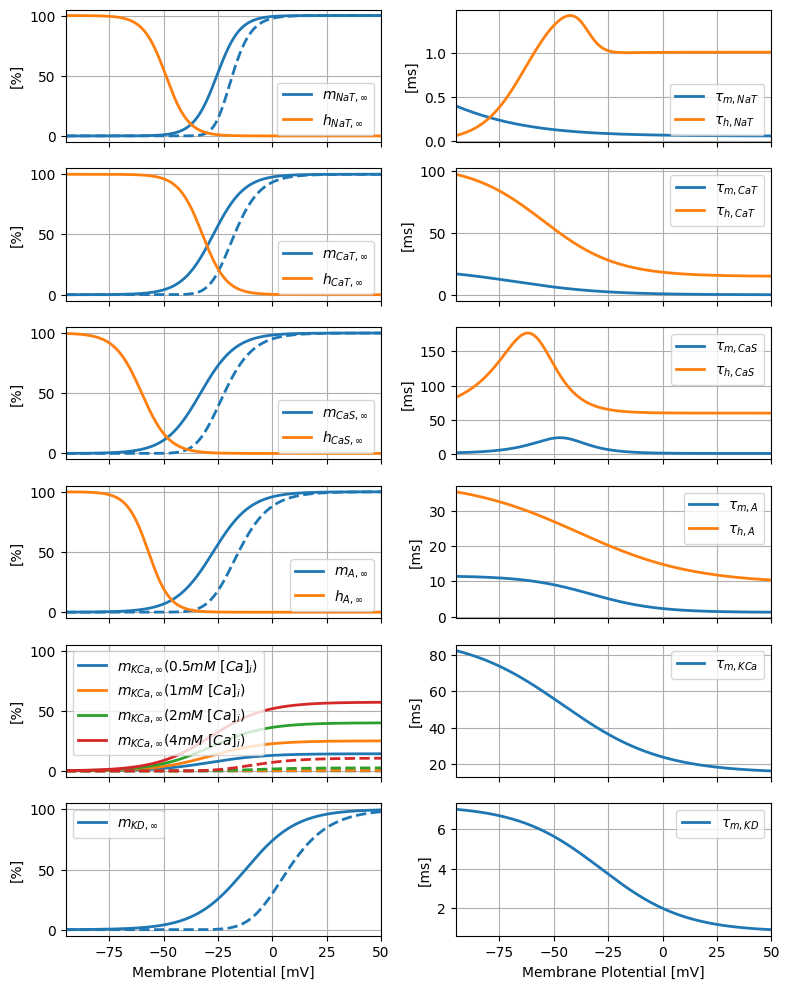
\includegraphics[width=\linewidth]{../img/model_kinetics/goldman.png}
    \caption[Park: Steady state activation and inactivation functions, and corresponding time constants]{
        \textbf{Park: Steady state activation and inactivation functions, and corresponding time constants} Parameters adapted from \parencite{parkMathematicalModelSubthalamic2021}.
    }
    \label{fig:kinetic_plots_park}
\end{figure}



%%%%%%%%%%%%%%%%%%%%%%%%%%%%%%%%%%%%%%%%%%%%%%%%%%%%%%%%%%%%%%%%%%%%%%%
\subsection{EAG Channel} \label{appendix:parameters_eag_channel}

\begin{table}[H]
    \centering
    \begin{tabular}{|l||c|c|c|}
    \hline
    \textbf{Model} & $a$ & $d$ & K$^+$ \\
    \hline
    \hline
    Default \parencite{bronkRegulationEagCa22018}  & $1$       & $0$        & $16.94$ \\
    Wang 1994     & $0.01$    & $-35.5$    & $0.2$  \\
    % Goldman 2001  & $1$       & $0$        & $4$    \\
    \hline
    \end{tabular}
    \caption{Parameter values for EAG channels used in implemented models.}
    \label{tab:eag_parameters}
\end{table}


\end{document}